\section{The I-MOVE Dataset}
Compared to the reviewed datasets, I-MOVE is unique in a number of characteristics. 
Firstly the dataset is the only in our knowledge that focuses on and provides object motion parameters, it also contains a larger number of industry-relevant objects and scenes with both indoor and outdoor data to help provide adequate data to create more robust models. 
The data is also captured with a variety of cameras from six different angles in order to ensure accuracy in ground truth and maximum effectiveness when conducting tests of researcher's models. 
The velocity ground truth is also thoroughly proofed and tested to ensure accuracy with physics based examples and settings to allow completely mathematical based calculations to be done by hand and compared against. 

\subsection{Setup}
The equipment setup used for the dataset was meticulously crafted to ensure the most reliable results possible when setting up and collecting data in various locations / scenes. 
The six cameras and two radars were mounted on a 14 gauge angle bar as can be seen in Figure~\ref{fig:RIG.png}.

\begin{figure}[t!]
    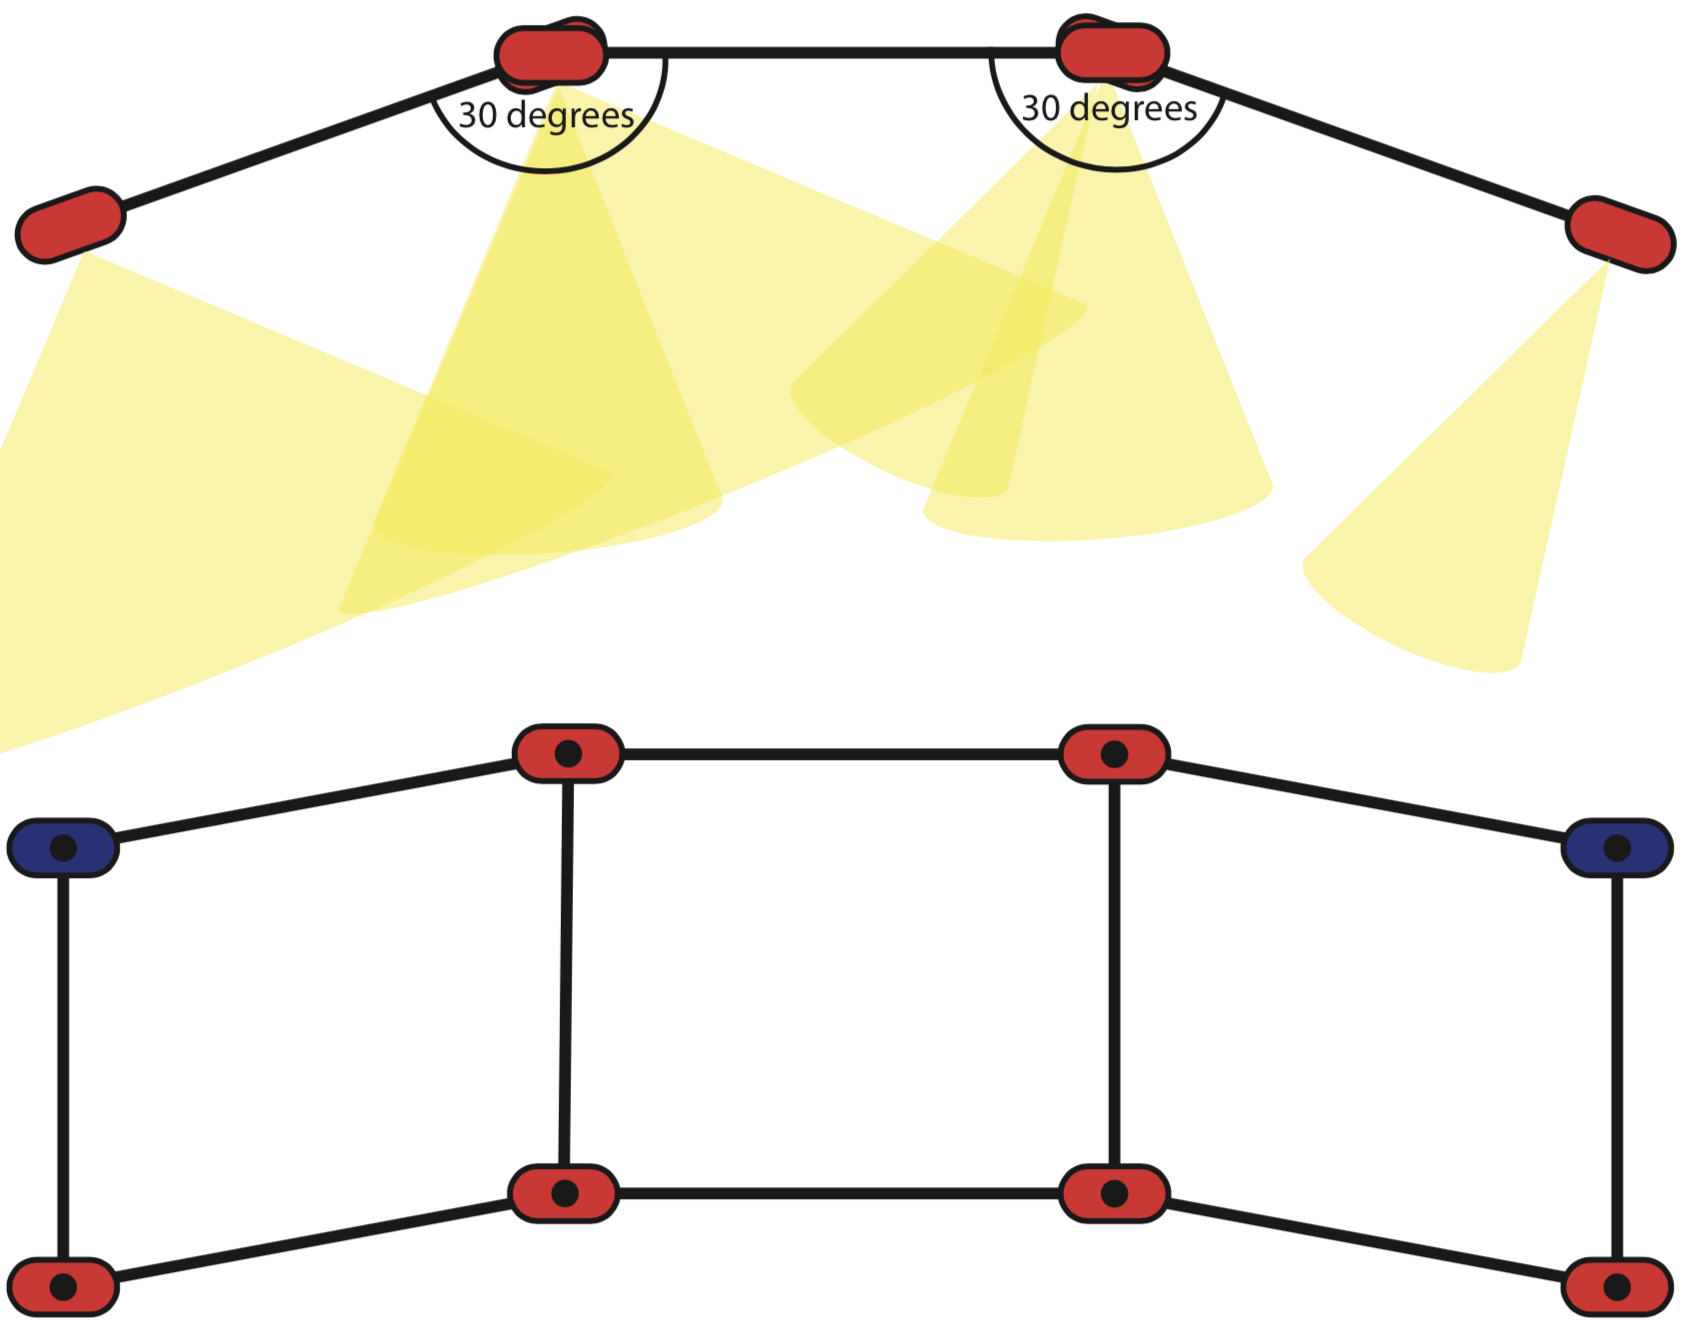
\includegraphics[width=\columnwidth]{Images/RIG.png}
    \caption{
    Above is the top view of the rig. each bar is 2 meters long and placed at a 30 degree difference from the other. The red rounded rectangles represent the cameras while the yellow represents the cameras' field of view. The field of view shrinks and pixel count increases as you go toward the right of the rig. The bottom is the front view of the rig as can be seen, there are six cameras represented by the red rounded rectangles and two radars represented by the blue rounded rectangles.
    }\label{fig:RIG.png} 
\end{figure}

The cameras and radars were mounted in the same order / setup for each location, to ensure appropriate comparisons can be made between different perspectives and camera effectiveness in different settings. 
The cameras used were three GoPro Hero 3 stereo rigs (six GoPros in total), along with two Intel RealSense cameras, a 415 and 435, and lastly a ZED camera. 
The radars used were OmniPreSense radars, which provide velocity of objects within their $78^{\circ}$ wide beams.

Due to the wide variety in lighting, size of objects and scene layouts / environments where data was collected the rig had to be created to accommodate these differences. 
The cameras all have a different degree of viewing capability so the order and spacing of them was vital to collect data as best possible. 
Two of the GoPro setups have modified lens giving them a field of view of $54.1^{\circ}$ for one of the modified setups and $64.7^{\circ}$ for the other.
The standard / unmodified GoPro stereo set up has a horizontal field of view of $122.6^{\circ}$.
The Intel RealSense 435 has a field of view of $85^{\circ}$ horizontally, while the RealSense 415 version has $63^{\circ}$, and finally, the ZED is capable of $90^{\circ}$ viewing horizontally.
Given our purposeful placement of the cameras we were able to obtain a two foot spacing between each camera allowing for fairly significant difference in camera perspective while still having all cameras capturing the object and it's most valuable movements. 
This can be seen in Fig ???

\subsection{Data Collection}
Our data collection process was intended to include a significant variety in objects, object motion, object velocity, scenes / environments and lighting, while still ensuring maximal accuracy in the ground truth for segmentation and velocity of the object.
The current dataset features ten different objects: person, car, dog, skateboarder, skateboard, biker, ball, drone, frisbee and RC Car. 
These objects differ widely not only in shape and size but also motion paths making them suitable to train and test upon. 

\subsection{Calculation and Verification of Velocity}
The main purpose of this dataset is to provide the necessary data to better predict motion parameters of an object. 
Because of this it is vital that the ground truth is as accurate as possible. 
To ensure the velocity of each object is correct we have additional purely physics based scenes put in place, some of these include dropping an object, rolling a ball down a ramp, and swinging a pendulum.
These can be seen in Figure\ref{fig:phys.png}

\begin{figure}[t!]
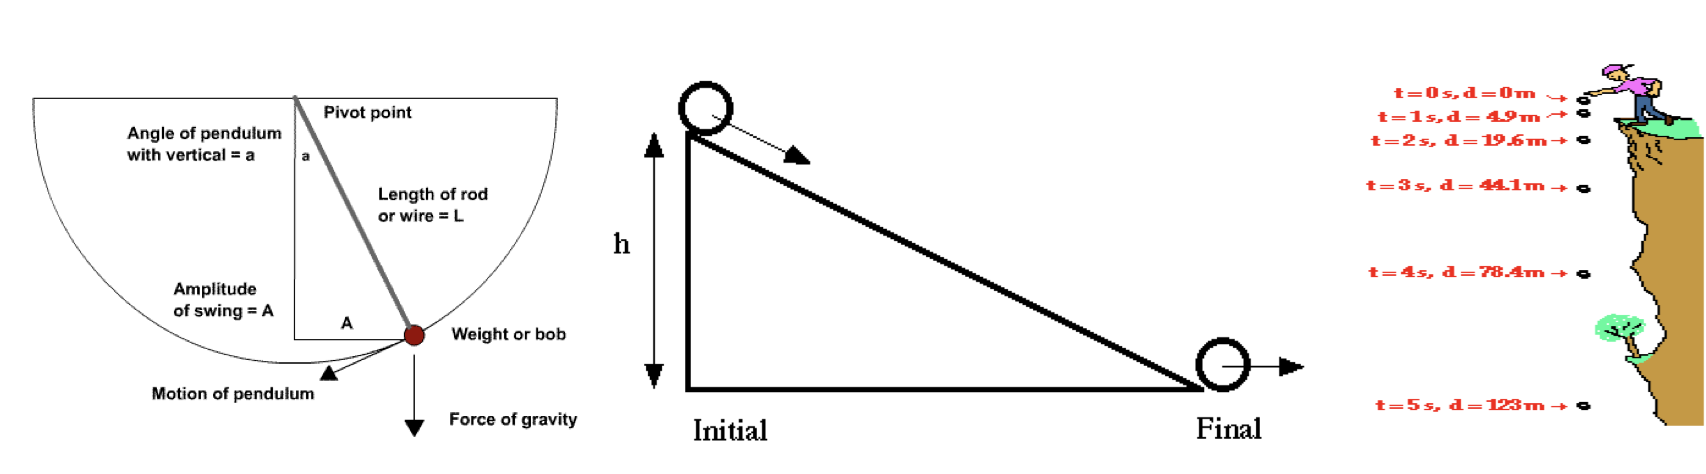
\includegraphics[width=\columnwidth]{Images/phys.png}
\caption{A schematic of the physics setups used for data collection. Pendulum seen on the left, rolling ball on incline in the middle, and dropping ball on the right.}\label{fig:phys.png} 
\end{figure}

The velocity data for the ball drop was computed using the commonly known equation $V = gt$ where gravity is 9.8 meters per second squared and t is the time since ball was released. The rolling ball's velocity at the end of the ramp / incline was calculated using the equation $V =  \sqrt{ \frac{10}{7}gh}$ where g is once again gravity and h is the height of the ramp. Finally the velocity of the pendulum was found using the equation $V =  \sqrt{2gL(1-cos(a)}$ where V is the velocity at the bottom of the swing, a is the angle from vertical, and L is length of the pendulum. These accompanied by hand calculated velocities using two OmniPreSense radars allow us to provide the most accurate velocities possible.

%\section{Segmentation Benchmark}
